\documentclass[]{report}
\usepackage{graphicx}
\usepackage{hyperref}


% Title Page
\title{Report on state of the art}
\author{Developing 3D molecular representation}

\begin{document}
\maketitle
\chapter{Cartesian coordinate}


\section{Learning a Continuous Representation of 3D Molecular Structures with Deep Generative Models}

Ragoza, Matthew \& Masuda, Tomohide \& Koes, David. (2020). Learning a Continuous Representation of 3D Molecular Structures with Deep Generative Models. 

\begin{enumerate}
	\item This work uses a deep generative models with atomic density grids and a fitting algorithm that converts the grids into discrete molecular structures. 
	\item Deep learning for generative modeling can be categorized into two types:
	\subitem An encoder and  decoder network
	\subitem Generative adverserial networks (GANs)
	\item Initially the deep generative models used SMILES format but there are problems like same molecules can have different SMILES strings. Invalid strings can be produced. SMILES is capable of representing only the connection between the molecules it can not represent 3D conformations.
	\item Not a lot of progress has been made in  3D molecular graph-based models.
	 \item Generative models seem to overcome the limitations of other models/ methods in machine learning and this paper uses a generative model for the generation and representation of 3D structures.
	 \subsection{Working}
	 \item Input = Molecules are encoded in a latent space using density grid. Molecules are translated to atom types and coordinates before being converted to atomic density grids.
	 \item A latent space is a representation of compressed data in which similar data points are grouped together.[1]
	 \item They are decoded in similar format.
	 \item An algorithhm is applied for fitting the 3D structures for generating atomic densities and valid molecules. Atom fitting is a technique for converting density to atom kinds and coordinates.
	 \item 	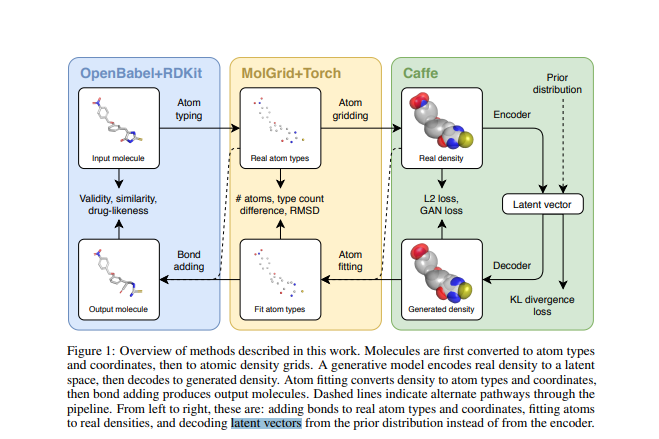
\includegraphics[width=\linewidth]{RND_reports/DGM.png}
	 \item This is the link that provides code for this model \href{ https://github.com/mattragoza/liGAN}{ https://github.com/mattragoza/liGAN} 
	 \item MolPort database is used for experimentation.
\end{enumerate}


\section{Machine learning based energy-free structure
predictions of molecules, transition states, and solids}

\begin{enumerate}
    \item This work uses supervised learning for addressing 3D molecular structures it's called Graph To Structure (G2S) model.
    \item State of the art approaches like ETKDG6 and Gen3D7 are efficient but not very general.
    \item Kernel ridge regression is used in G2S model. It is for the prediction of all elements in the pairwise distance matrix. This matrix is used for re-creating the atomic coordinates of molecules. 
    \item Kernel ridge regression (KRR) combines ridge regression (linear least squares with l2-norm regularization) with the kernel trick.[2]
    \item Model only accepts stoichiometry based information as input.
   
    \subsection{Working}	
    \item First step is to separate hydrogen atoms and heavy molecules.
    \item Molecular bonding patterns are converted into graph representation of fixed size.
    \item One model per distance-pair is used for calculating pair- wise distance. 
    \item For the prediction of interatomic distances for out-of-sample molecules, only information related to bonding pattern and nuclear charges is needed.
    \item RDkit is used to create adjacency matrix which is later used for representations.
    \item The distance geometry problem occurs when inter-atomic distances are converted to 3D coordinates. DGSOL15 is used for heavier atoms.
    \item The problem of distance geometry is not related to the model.
    \item QM9 database is used.
	 \item 	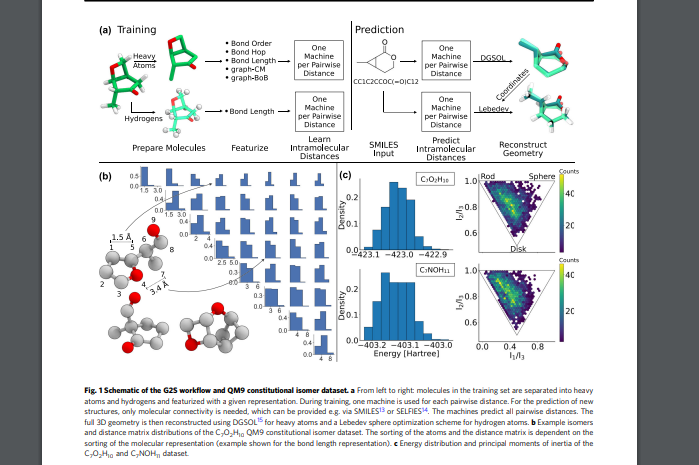
\includegraphics[width=\linewidth]{RND_reports/G2S.png}
	 \item The code for this model is :\href{https://zenodo.org/record/4792292#.YZvsq5HMLRY}{Website of this model}
\end{enumerate}
	 
	 
	
\section{3D-TRANSFORMER: MOLECULAR REPRESENTATION WITH TRANSFORMER IN 3D SPACE}
\begin{enumerate}
    \item This work presents a 3D Transformer which takes 3D coordinates and the types of atoms as input. It works on fully-connected graph. 
    \item It contains a a Multi-scale Self-Attention module for finding the patterns from neighbourhoods.
\end{enumerate}
	 
\section{Dataset’s chemical diversity limits
the generalizability of machine learning
predictions}
\begin{enumerate}
    \item This work presents a comparative analysis using QM9 and a new data set PC9. The problem they are trying to address is generalization of datasets for testing them on different ML models.
    \item The models used in this paper are: Kernel ridge regression (KRR), Elastic net Elastic Net, SchNet neural networks.
    \item The models were assessed for a few energetic properties like :
    \subitem total molecular energy E 
    \subitem energy of HOMO 
    \subitem energy of LUMO 
    \item The atomization energies were used in the modeling for all the ML models.
    \item The models were trained on one of the datasets and one for prediction.
    \item For molecular representation Coulomb Matrix (CM)  is used.
    \item Other ways for molecular representations are:
    \subitem Graph representations 
    \subitem  Coulomb Matrix 
    \subitem Bag of Bonds (BoB)
    \subitem Bonds and Angles ML (BAML) descriptors 
    \item CM is a square atom by atom matrix constructed from atomic nuclear charges (Z) and Cartesian coordinates of each atom (R)[3]
    \item Coulomb Matrix Eigenvalues (CME) are a global 3-dimensional representation of molecular structure,
which have been previously used to predict atomization energies, prioritize geometry searches, and
interpret rotational spectra. The properties of the CME representation and its relationship to molecular
structure are established using the Gershgorin circle theorem. [4]
\item EN, KNN and SchNet were tested for QM9 first and then for PM9.  All models obtain lower accuracy on PC9 data than they do on QM9 data.
\end{enumerate}

	
\section{Applying machine learning
techniques to predict the properties
of energetic materials}
\begin{enumerate}
    \item 2018 Paper
    \item This work presents a comparison between molecular featurization method and ML models . 
    \item Their aim is to create a network model that predicts the energetic properties.
    \item Featurization is the process to convert varied forms of data to numerical data which can be used for basic ML algorithms.[5]
    \item Different featurization techniques are:
    \subitem Custom descriptor set
    \subitem Sum over bonds
    \subitem Coulomb matrices
    \subitem Bag of bonds
    \subitem Fingerprinting
    \subitem Atom-Pair
    \subitem Topological Torsion
    \subitem Extended Connectivity Fingerprints (ECFPs)
    \subitem E-state fingerprints
    \subitem Avalon fingerprints
    \subitem RDKit graph fingerprints
    \subitem ErG fingerprints
    \subitem physiochemical property
    \subitem 
fingerprints.
    \subitem SOAP and Fourier series of atomic radial distribution functions. Both of these methods had poor performance.
    \item A few built in featurization vectors for neural networks are:
    \subitem custom graph convolutional fingerprints
    \subitem deep tensor networks
    \subitem 5 message
passing neural networks
    \subitem hierarchically interacting particle neural nets.
    \subitem

\end{enumerate}

	
\section{A Chemical Bond-Based Representation of Materials}
\begin{enumerate}
    \item This work presents a new method for representation which uses the chemical bond energy. 
    \item It aims at the prediction of atomization energies by using machine learning. 
    \item related work includes Coulomb Matrix and orbital-field matrix.
\end{enumerate}


\section{Constant size descriptors for accurate machine learning models of molecular properties}
\begin{enumerate}
    \item This work presents a discussion on two different ways or classes of molecular representation for an ML model.
    \item For the first class requirements include : 
    A graph of the molecular structure.
    The count of the occurrences of bonding pattern. The advantage is that these can be extracted from a single line of SMILES.
    \item Second class requires 3D structure of the molecule. This class consists of Coulomb matrix, Bag of Bonds, and Bonds and Angles Machine Learning. features. The model is efficient at predicting molecular properties such as thermodynamics and electronic properties. 
    \subitem If the number of interactions increase in a molecule then the length of feature vector increases. 
    \item A constant size geometry feature vector was introduced as well. It is similar to Coulomb matrix or BOB. The purpose of this feature vector, whose length is independent of molecular size, it to generalize the models.
    \item For assessment kernel-based learning ML models have been used. With QM7 dataset.
    \item \textbf{KRR performs better over LRR} using different feature vectors.
\end{enumerate}

	
\section{Structure-Based de Novo Molecular Generator Combined with Artificial Intelligence and Docking Simulations}
\begin{enumerate}
    \item This work presents a new design method for generating molecules by implementing a recurrent neural network, and a Monte Carlo tree search along with docking simulations.\textbf{SBMolGen}
    \item The models aims to generate molecules with better affinity score and compare them.
    \item The binding affinity is the strength of the interaction between two (or more than two) molecules that bind reversibly (interact).[6]
    \item It uses SMILES as input for the model for generation of molecules.
    \item After experimentation it was observed that the molecules that were generated has similar structural and physiochemical properties as previously known drugs.
    \item The model was successful in creating new molecules and future work can be related to improving the computational time.
    \item 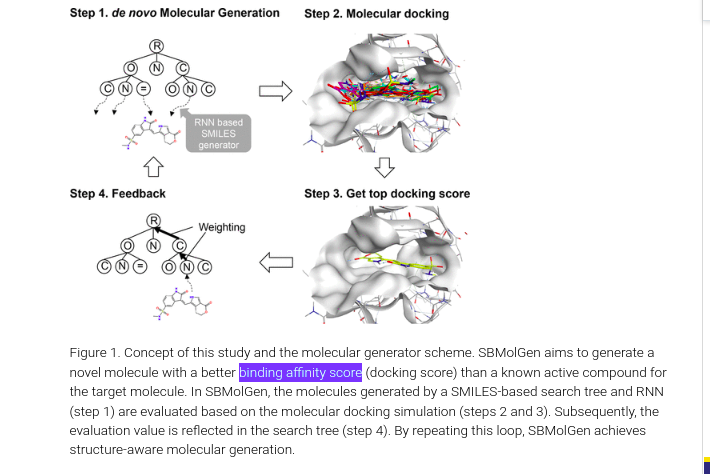
\includegraphics[width=\linewidth]{RND_reports/affinity_score.png}
    \item 
\end{enumerate}







\chapter{Z- Matrix}

\section{Z-matrix template-based substitution approach
for enumeration of 3D molecular structures}
Wanutcha Lorpaiboon, Taweetham Limpanuparb,
Z-matrix template-based substitution approach for enumeration of 3D molecular structures,
MethodsX,
Volume 8,
2021,
101416,
ISSN 2215-0161,
https://doi.org/10.1016/j.mex.2021.101416.
(https://www.sciencedirect.com/science/article/pii/S2215016121002090)
\begin{enumerate}
    \item Z matrix and Cartesian coordinates are two ways of  molecular representation. Both these ways can be inter converted using software. 
    \item Z matrix consists of more information related to molecules e.g bond lengths, bond angles and torsional angles,
    \item This paper aims to represent different conformations molecules in 3D.
    \item Collection of halo substituted benzene are demonstrated in this paper.
    \item Initially Z matrix is used in lower strings.
    \item IQmol is used to construct the initial template.
    \item The template can be calculated by hand too.
    \item With the help of Wolfram Mathematica notebook tuples are generated and then similar tuples are remove.
    \item The final tuples are converted to SMILES format.
    \item This template replacement method can result in a variety of compounds of the same class.
    \item This was only for basics. It does not use any ML model. It is for training in classrooms.
\end{enumerate}





\section{References}
1. https://towardsdatascience.com/understanding-latent-space-in-machine-learning-de5a7c687d8d

2. https://scikit-learn.org/stable/modules/generated/sklearn.kernel ridge.KernelRidge.html

[3]. Glavatskikh, Marta & Leguy, Jules & Hunault, Gilles & Cauchy, Thomas & Da Mota, Benoit. (2019). Dataset’s chemical diversity limits the generalizability of machine learning predictions. Journal of Cheminformatics. 11. 10.1186/s13321-019-0391-2. 
[4] @article{Schrier2020CanOH,
  title={Can One Hear the Shape of a Molecule (from its Coulomb Matrix Eigenvalues)?},
  author={Joshua Schrier},
  journal={Journal of chemical information and modeling},
  year={2020}
}
[5] https://www.kaggle.com/general/223108
[6] https://royalsocietypublishing.org/doi/10.1098/rsif.2012.0835
\end{document}          
